
\section{Geração dos Dados}\label{Metodologia.}

O projeto proposto será composto pelas etapas que seguem (\autoref{fig_fluxo_met}), sendo que neste capítulo, trata-se da geração de dados e execução. Foram geradas três instâncias para a análise da rede logística. 

\begin{figure}[htb]
	\caption{\label{fig_fluxo_met} Fluxo logístico do envio e retorno de maquinetas, laço fechado}
	\begin{center}
            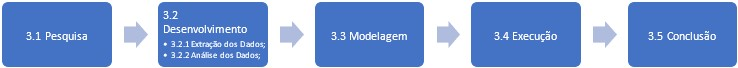
\includegraphics[width=15cm]{images/RF_img/FluxoMetodologia.jpg}
	\end{center}
	\fdadospesquisa
\end{figure}


 


A implementação detalhada do código-fonte está disponível no Apêndice \ref{anexo:codigo}, através de um link para o github.


%\subsection[Pesquisa]{Pesquisa}
%\label{Pesquisa}
%Esta etapa se trata da pesquisa por mais projetos desenvolvidos no assunto abordado, pela revisão bibliográfica de mais artigos e exemplos de sucesso no desenvolvimento e escrita/documentação do que foi estudado.

%Esta etapa se trata da pesquisa por mais projetos desenvolvidos no assunto abordado, pela revisão bibliográfica de mais artigos e exemplos de sucesso no desenvolvimento e escrita/documentação do que foi estudado.

%\subsection[Desenvolvimento]{Desenvolvimento}
%\label{Desenvolvimento}

%Para o desenvolvimento do estudo, devido a capacidade computacional, as análises foram reduzidas para o estado de SP como validação do modelo.

\subsection{Geração de Dados e Definições de Parâmetros}
\label{Extração dos Dados}

Nesta etapa, foram coletados dados de estados, regiões, regiões imediatas, municípios, latitude, longitude e população por município diretamente da \sigla{API}{Interface de Programação de Aplicativos} do \sigla{IBGE}{Instituto Brasileiro de Geografia e Estatística} \cite{ibge:2025:divisoesregionais} (\autoref{tab:dados_municipios}).

\begin{table}[h!]
\centering
\caption{Características das Colunas de Dados dos Municípios Brasileiros}
\label{tab:dados_municipios}
\begin{tabular}{|p{5cm}|p{2cm}|p{2cm}|p{5cm}|} % Ajuste das larguras das colunas
\hline
\textbf{Coluna} & \textbf{Número de Linhas} & \textbf{Tipo} & \textbf{Descrição} \\
\hline
uf & 645 & object & Sigla do estado \\
\hline % Linha adicionada
regiao & 645 & object & Região do Brasil \\
\hline % Linha adicionada
codigo\_ibge & 645 & object & Código único do município \\
\hline % Linha adicionada
nome\_cidade & 645 & object & Nome da cidade \\
\hline % Linha adicionada
latitude\_cidade & 645 & float64 & Latitude da cidade \\
\hline % Linha adicionada
longitude\_cidade & 645 & float64 & Longitude da cidade \\
\hline % Linha adicionada
Nome do Município & 645 & object & Nome da cidade \\
\hline % Linha adicionada
Nome da Região Imediata & 645 & object & Nome da região geográfica imediata \\
\hline % Linha adicionada
Nome do Município da Região Imediata & 645 & object & Nome do principal município da região geográfica imediata \\
\hline % Linha adicionada
Pop\_2022 & 645 & float64 & População estimada para 2022 \\
\hline
\end{tabular}
\end{table}

%\subsubsection[Geração de Dados e Definições de Parâmetros]{Geração de Dados e Definições de Parâmetros}
%\label{Geração de Dados}\par

Para o teste das instâncias, foram gerados os parâmetros correspondentes ao modelo apresentado na Seção \ref{Modelagem Matemática}. Seguindo a estrutura metodológica, os dados de entrada encontram-se segmentados por clientes, PAs, CDs e fábrica. Como elemento central para a minimização da função objetivo, destacam-se os parâmetros financeiros associados aos custos fixos de abertura e manutenção das facilidades logísticas, bem como o custo de transporte por máquina e por quilômetro rodado, conforme sumarizado na \autoref{tab:parametros_custos}.

\begin{table}[h!]
\centering
\caption{Parâmetros de custos do sistema logístico}
\label{tab:parametros_custos}
\begin{tabular}{|c|l|c|}
\hline
\textbf{Símbolo} & \textbf{Descrição} & \textbf{Valor (R\$)} \\
\hline
$h_{i}$ & Custo de abertura de Centro de Distribuição (CD) & 3.000.000 \\
\hline
$v_{i}$ & Custo anual de manutenção de Centro de Distribuição (CD) & 100.000 \\
\hline
$u_{p}$ & Custo de abertura de Posto Avançado (PA) & [3.000, 864.000]* \\
\hline
$x_{p}$ & Custo anual de manutenção de Posto Avançado (PA) & [150, 43.200]* \\
\hline
$k$ & Custo de transporte por quilômetro por unidade & 0,015 \\
\hline
\end{tabular}
\end{table}

\subsubsection{Clientes - Zonas de Demanda (ZDs)}
\label{Clientes}

Os parâmetros para clientes basicamente são dois: demanda de instalação e demanda de desinstalação \autoref{tab:clientes}. Os dados de demanda estão por latitude e longitude, sendo dados gerados através dos dados de população, que foi extraída conforme na seção \ref{Extração dos Dados}.\par

\begin{table}[h!]
\centering
\caption{Clientes}
\label{tab:clientes}
\begin{tabular}{|c|c|c|c|}
\hline
\textbf{Variável} & \textbf{Instância 1} & \textbf{Instância 2} & \textbf{Instância 3} \\
\hline
$dem^{rj}_{j,t}$ & $dem^{rj}_{j,t} \in [0, 1.146M]$ & $dem^{rj}_{j,t} \in [0, 1.172M]$ & $dem^{rj}_{j,t} \in [0, 1.179M]$ \\
\hline
$dem^{aj}_{j,t}$ & $dem^{aj}_{j,t} \in [0, 1.322M]$ & $dem^{aj}_{j,t} \in [0, 1.362M]$ & $dem^{aj}_{j,t} \in [0, 1.367M]$ \\
\hline
\end{tabular}
\end{table}

Inicialmente foi gerado um histograma para classificar os municípios conforme sua população, utilizando a faixa de 50 mil habitantes como critério principal. A visualização dessa classificação pode ser encontrada na Figura \ref{fig_hist_c_sp}.

\begin{figure}[htb]
	\caption{\label{fig_hist_c_sp} Histograma da população do estado de São Paulo}
	\begin{center}
            \includegraphics[width=10cm]{images/RF_img/Pop_c_SP_Hist.png}
	\end{center}
	\fdadospesquisa
\end{figure}

O estado de São Paulo possui uma concentração muito grande e discrepante na capital em relação às outras cidades, tendo sua faixa populacional acima de 12 milhões de habitantes. Com isso, foi necessário um tratamento à parte, sendo criado um novo histograma sem a cidade de São Paulo, utilizando faixa populacional de 25 mil habitantes \autoref{fig_hist_s_sp}.

\begin{figure}[htb]
	\caption{\label{fig_hist_s_sp} Histograma da população do estado de São Paulo sem a capital}
	\begin{center}
            \includegraphics[width=10cm]{images/RF_img/Pop_s_SP_Hist.png}
	\end{center}
	\fdadospesquisa
\end{figure}

A geração da demanda foi realizada através da demanda total de maquinetas, que foi de 20 milhões em um ano; em seguida, a empresa que está sendo analisada possui um \emph{market share} (percentual de participação do mercado) de 30\%, com isso foi aplicado este percentual definindo a demanda anual da empresa em questão. Calcula-se a média mensal e aplica-se uma variação randômica seguindo uma distribuição normal com variação de 10\%.

A demanda considerada foi limitada ao estado de SP devido a restrições computacionais, totalizando cerca de 1,3 milhão de instalações anuais, com média de 110 mil por mês. Em função da LR da cadeia, a demanda de desinstalação é estimada em 80\% da demanda de instalação. A Figura \ref{grafico_demanda_isnt_desinst_01} apresenta as curvas de demanda anual (instalação e desinstalação) para a instância 1.

\begin{figure}[htb]
	\caption{\label{grafico_demanda_isnt_desinst_01} Gráfico de Demanda de Instalação e Desinstalação para o Estado de São Paulo - Instância 1}
	\begin{center}
            \includegraphics[width=10cm]{images/RF_img/Demanda_linha_inst_01.png}
	\end{center}
	\fdadospesquisa
\end{figure}

A Instância 2 simula a sazonalidade de Natal, aplicando um acréscimo de 20\% na demanda de instalação em dezembro. Em função da LR e do volume instalado, a demanda de desinstalação apresenta um aumento correspondente de 20\% em janeiro. O perfil da demanda desta instância está detalhado na Figura \ref{grafico_demanda_isnt_desinst_02}.

\begin{figure}[htb]
	\caption{\label{grafico_demanda_isnt_desinst_02} Gráfico de Demanda de Instalação e Desinstalação para o Estado de São Paulo - Instância 2}
	\begin{center}
            \includegraphics[width=10cm]{images/RF_img/Demanda_linha_inst_02.png}
	\end{center}
	\fdadospesquisa
\end{figure}

Para a instância 3, é aplicado uma sazonalidade para o período de carnaval, ocorrendo um aumento de 20\% na instalação no mês de fevereiro e o mesmo aumento de 20\% na desinstalação de março, em decorrência do aumento ocorrido na instalação no mês anterior (\autoref{grafico_demanda_isnt_desinst_03}).

\begin{figure}[htb]
	\caption{\label{grafico_demanda_isnt_desinst_03} Gráfico de Demanda de Instalação e Desinstalação para o Estado de São Paulo - Instância 3}
	\begin{center}
            \includegraphics[width=10cm]{images/RF_img/Demanda_linha_inst_03.png}
	\end{center}
	\fdadospesquisa
\end{figure}

As demandas foram contabilizadas por cidade, porém para melhorar o processamento computacional, a demanda foi consolidada em ZDs. Para definir essas zonas, foram selecionadas 50\% das cidades com maior demanda e com isso a demanda restante foi redistribuída entre estas cidades proporcionalmente. Com isso houve uma redução em 50\% da base de dados total.

% Desta maneira, a distribuição das ZDs por faixa de demanda é apresentada conforme \autoref{hist_faixa_cidade_01}, percebe-se que 5 ZDs possuem o volume muito alto, enquanto as demais são mais uniformemente distribuídas para a instância 1 e .

% \begin{figure}[htb]
% 	\caption{\label{hist_faixa_cidade_01} Histograma de Cidades por Faixa Demanda }
% 	\begin{center}
%             \includegraphics[width=10cm]{images/RF_img/Faixa_Dem_Cidades_inst_01.png}
% 	\end{center}
% 	\fdadospesquisa
% \end{figure}\par

% \begin{figure}[htb]
% 	\caption{\label{hist_faixa_cidade_02} Histograma de Cidades por Faixa Demanda }
% 	\begin{center}
%             \includegraphics[width=10cm]{images/RF_img/Faixa_Dem_Cidades_inst_02.png}
% 	\end{center}
% 	\fdadospesquisa
% \end{figure}\par

% \begin{figure}[htb]
% 	\caption{\label{hist_faixa_cidade_03} Histograma de Cidades por Faixa Demanda }
% 	\begin{center}
%             \includegraphics[width=10cm]{images/RF_img/Faixa_Dem_Cidades_inst_03.png}
% 	\end{center}
% 	\fdadospesquisa
% \end{figure}\par



\subsubsection{Postos Avançados (PAs)}
\label{Postos Avançados}

Para os PAs, foram identificadas algumas cidades com potencial para implantação, com base nas Regiões Geográficas Imediatas. De acordo com o \citeonline{ibge:2024:compreendendoterritorio}, essas regiões representam áreas cujos habitantes recorrem a centros urbanos próximos para suprir necessidades imediatas, como acesso a emprego, saúde, educação, consumo e serviços públicos. Dentro de cada região imediata, foram selecionadas as duas maiores cidades, obtendo-se um total de 112 cidades conforme apresentado na \autoref{poss_pa_sp}.

\begin{figure}[htb]
	\caption{\label{poss_pa_sp} Mapa com as possíveis cidades para abertura de um PA.}
	\begin{center}
            \includegraphics[width=10cm]{images/RF_img/poss_pa_sp.png}
	\end{center}
	\fdadospesquisa
\end{figure}

Para as instâncias 1,2 e 3, o parâmetro $n^{p}$ (quantidade máxima de aberturas de PAs) foi definido como 70\% do total de cidades elegíveis à instalação de um PA. O parâmetro $e^{p}_{p,t}$ (limite máximo de máquinas em estoque) foi determinado individualmente para cada possível PA, com base na faixa de demanda da respectiva região imediata, sendo fixado em 125\% do valor da faixa de maior demanda. Esse critério visa garantir um estoque suficiente para cobrir até 36 dias de operação do PA.

Os parâmetros $m^{rp}_{p}$ (capacidade máxima de recebimento no PA) e $m^{ap}_{p}$ (capacidade máxima de envio do PA) foram estipulados como aproximadamente 80\% do estoque inicial, assegurando o atendimento da demanda estimada para um período de 30 dias. O parâmetro $c^{pj}_{p,j}$ (indicador de pertencimento regional entre os PAs e as ZDs) assume sempre o valor 1, uma vez que o modelo foi restrito ao estado de São Paulo; portanto, todas as ZDs pertencem ao mesmo estado onde os PAs podem ser implantados.

O cálculo do parâmetro de distância $d^{pj}_{p,j}$ (entre os PAs e as ZDs) é realizado utilizando-se a \textbf{distância euclidiana}, a partir das coordenadas geográficas (latitude e longitude) dos respectivos pontos, conforme especificado na \autoref{tab:parametros_pa}.

Esta opção metodológica se justifica pela indisponibilidade de uma base de dados fidedigna que contenha as distâncias rodoviárias reais entre os municípios do estado de São Paulo. É importante ressaltar que a utilização da distância euclidiana implica uma simplificação do problema, não incorporando fatores do mundo real, como rotas específicas ou cobranças por pedágio.

\begin{table}[h!]
\centering
\caption{Parâmetros PA}
\label{tab:parametros_pa}
\begin{tabular}{|c|c|}
\hline
\textbf{Parâmetro} & \textbf{Instância 1, 2 e 3} \\
\hline
$n^{p}$ & 112 \\
\hline
$e^{p}_{p,t}$ & $e^{p}_{p,t} \in [550, 176.300]$ \\
\hline
$m^{rp}_{p}$ & $m^{rp}_{p} \in [275, 88.150]$ \\
\hline
$m^{ap}_{p}$ & $m^{ap}_{p} \in [275, 88.150]$ \\
\hline
$c^{pj}_{p,j}$ & 1 \\
\hline
$d^{pj}_{p,j}$ & $d^{pj}_{p,j} \in [0, 830]$ \\
\hline
\end{tabular}
\end{table}

\subsubsection{Centros de Distribuição (CDs)}
\label{Centros de Distribuição}

A seleção das cidades para a possível instalação de Centros de Distribuição (CDs) considerou diversos critérios estratégicos: proximidade com aeroportos, infraestrutura adequada para operações logísticas, reconhecimento histórico como polos logísticos, além da localização próxima à fábrica e à empresa responsável pelos descartes. As cidades escolhidas foram: Americana, Guarulhos, Hortolândia, Jundiaí, Mogi das Cruzes, Osasco, São José dos Campos, Sorocaba e Suzano (\autoref{poss_cd_sp}).

\begin{figure}[htb]
	\caption{\label{poss_cd_sp} Mapa com as possíveis cidades para abertura de um PA.}
	\begin{center}
            \includegraphics[width=10cm]{images/RF_img/poss_cd_sp.png}
	\end{center}
	\fdadospesquisa
\end{figure}

O parâmetro $e^{c}_{i,t}$ (limite máximo de máquinas em estoque) é calculado com um acréscimo de 20\% sobre o estoque inicial de 200 mil máquinas — sendo 100 mil aptas para uso e 100 mil destinadas ao descarte ou reparo na fábrica. Esse valor de 100 mil foi estabelecido com o objetivo de garantir atendimento à demanda por um período de 30 dias.

Os parâmetros $m^{rc}{i}$ (limite máximo de recebimento de máquinas no CD) e $m^{ac}{i}$ (limite máximo de envio de máquinas pelo CD) são definidos com base nas capacidades operacionais esperadas do centro.

O parâmetro $c^{cp}_{i,p}$, que funciona como um indicador binário de pertencimento regional entre os CDs e os PAs, é fixado em 1, dada a premissa de que todas as instalações estão localizadas na mesma unidade federativa.

As distâncias $d^{cd}_{i,d}$ (entre os CDs e os pontos de descarte) e $d^{cp}_{i,p}$ (entre os CDs e os PAs) são calculadas utilizando-se a \emph{distância euclidiana}, a partir de suas coordenadas geográficas (latitude e longitude).

Por fim, o parâmetro $r^{c}$, que representa o fator de reenvio (ou proporção) para os CDs das máquinas recebidas dos PAs, é definido como $0,7$.  

\begin{table}[h!]
\centering
\caption{Parâmetros do CD}
\label{tab:parametros_cd}
\begin{tabular}{|c|c|}
\hline
\textbf{Variável} & \textbf{Instância 1, 2 e 3} \\
\hline
$n^{c}$ & 1, 2 e 3 \\
\hline
$e^{c}_{i,t}$ & 230.000 \\
\hline
$m^{rc}_{i}$ & 82.500 \\
\hline
$m^{ac}_{i}$ & 82.500 \\
\hline
$c^{cp}_{i,p}$ & 1 \\
\hline
$d^{cd}_{i,d}$ & $d^{cd}_{i,d} \in [0, 659]$ \\
\hline
$d^{cp}_{i,p}$ & $d^{cp}_{i,p} \in [4, 109]$ \\
\hline
$r^{c}$ & 0,7 \\
\hline
\end{tabular}
\end{table}

\subsubsection{Fábrica}
\label{Fábrica}

Os parâmetros empregados na configuração das Instâncias 1, 2 e 3 são idênticos, uma vez que foram obtidos a partir do histórico operacional fornecido pela empresa. Entretanto, a análise dos dados revela que a capacidade de envio e recebimento atribuída à fábrica é proporcionalmente inferior quando comparada aos demais pontos de estoque. Essa diferença se justifica pela função primária da fábrica, que é focada na produção e reparo das maquinas, e não na gestão de grandes volumes logísticos de distribuição.

\begin{table}[h!]
\centering
\caption{Parâmetros do Fabricante}
\label{tab:parametros_fabricante}
\begin{tabular}{|c|c|}
\hline
\textbf{Parâmetro} & \textbf{Instâncias 1, 2 e 3} \\
\hline
$m^{rf}_{l}$ & 11.700 \\
\hline
$m^{af}_{l}$ & 11.700 \\
\hline
$e^{f}_{l,t}$ & 62.404 \\
\hline
$c^{fc}_{l,i}$ & $c^{fc}_{l,i} \in [0, 1]$ \\
\hline
$d^{fc}_{l,i}$ & $d^{fc}_{l,i} \in [5, 102]$ \\
\hline
$r^{f}$ & 0,2 \\
\hline
\end{tabular}
\end{table}



\subsection{Análise dos Dados}
\label{Análise dos Dados}

Analisando o mapa de calor, com as divisões das regiões imediatas do estado de SP, percebe-se que há uma concentração populacional em torno da capital, com isso a demanda também se concentra nesta região, além de nestas regiões os PAs serem maiores, pois para o atendimento da demanda em regiões que possuem maior demanda, o parâmetro indica PAs com capacidade maior de atendimento. \autoref{fig_mapa_pop_sp}. 

\begin{figure}[htb]
	\caption{\label{fig_mapa_pop_sp} Mapa de calor populacional do estado de São Paulo}
	\begin{center}
            \includegraphics[width=14cm]{images/RF_img/Mapa_Pop_SP.png}
	\end{center}
	\fdadospesquisa
\end{figure}

\section[Resultados da Otimização e Comparativo de Custos]{Resultados da Otimização e Comparativo de Custos}

O modelo de Programação Linear Inteira Mista (PLIM) proposto foi implementado utilizando a linguagem de programação \textbf{Python 3.11} e resolvido pelo \emph{solver} \textbf{Gurobi Optimizer} na \textbf{versão 12.0.2} (build \texttt{v12.0.2rc0}, \texttt{win64}), reconhecido por sua alta eficiência na resolução de problemas de grande escala.

\subsection{Ambiente Computacional e Configuração do \emph{Solver}}

Os experimentos computacionais foram realizados em um \emph{laptop} com sistema operacional \textbf{Windows 11} (versão 11.0), equipado com um processador \textbf{AMD Ryzen 7 5700U with Radeon Graphics} e arquitetura \texttt{[SSE2|AVX|AVX2]}. Para o processamento das instâncias, o \emph{solver} foi configurado para utilizar \textbf{4 \emph{threads}} de um total de 16 processadores lógicos (8 núcleos físicos) disponíveis.

A Tabela \ref{tab:parametros_gurobi} apresenta os principais parâmetros não-padrão configurados no \emph{solver} Gurobi para todas as execuções.

\begin{table}[htb]
    \centering
    \caption{Parâmetros Não-Padrão do Gurobi Optimizer}
    \label{tab:parametros_gurobi}
    \begin{tabular}{lcl}
        \toprule
        \textbf{Parâmetro} & \textbf{Valor} & \textbf{Descrição} \\
        \midrule
        \texttt{TimeLimit} & $\texttt{7200}$ & Tempo máximo de execução de 7200 segundos (2 horas). \\
        \texttt{MIPGap} & $\texttt{0.05}$ & Tolerância de \emph{gap} de otimalidade de 5\% (5.00e-02). \\
        \texttt{Threads} & $\texttt{4}$ & Número de \emph{threads} alocados. \\
        \texttt{Presolve} & $\texttt{2}$ & Nível agressivo de pré-processamento. \\
        \texttt{Method} & $\texttt{1}$ & Utilização do algoritmo \emph{Dual Simplex} para a fase linear. \\
        \texttt{NodefileStart} & $\texttt{5}$ & Início do armazenamento de nós em arquivo (padrão implícito de 5 GB). \\
        \bottomrule
    \end{tabular}
\end{table}

\subsection{Dimensão do Modelo e Desempenho Computacional}

O modelo de otimização resultante apresentou uma estrutura de grande porte, com dimensões médias consistentes em todas as instâncias: $2.571.077$ restrições (\emph{rows}), $1.298.196$ variáveis (\emph{columns}) e $8.099.220$ elementos não-nulos. Dentre as variáveis, $865.104$ são contínuas e $433.092$ são inteiras (binárias).

O pré-processamento (\emph{Presolve}) demonstrou eficácia, removendo consistentemente cerca de $44$ mil linhas e $21$ mil colunas do modelo antes da otimização.

Em todas as instâncias, o \emph{solver} Gurobi encontrou uma \textbf{solução factível e de boa qualidade dentro da tolerância} estabelecida pelo parâmetro \texttt{MIPGap}. A Tabela \ref{tab:desempenho_resumo} consolida os principais resultados de desempenho para o conjunto de instâncias:

\begin{table}[h!]
\centering
\caption{Resumo do desempenho computacional e convergência por instância}
\label{tab:desempenho_resumo}
\begin{tabular}{|c|c|c|c|}
\hline
\textbf{Variável} & \textbf{Instância 1} & \textbf{Instância 2} & \textbf{Instância 3} \\
\hline
Gap de Otimização (\%) & 4,5257\% & 4,7284\% & 4,6818\% \\
\hline
Tempo de Execução & 3.687,98s (1,02h) & 3.722,30s (1,03h) & 3.877,71s (1,08h) \\
\hline
\end{tabular}
\end{table}

Os resultados obtidos para o \emph{gap} de otimalidade (variando entre $4,5257\%$ e $4,7284\%$) confirmam que as soluções alcançadas estão dentro da margem de $5\%$ exigida. O tempo de execução, com um máximo de $3.877,71$ segundos (aproximadamente 1 hora e 4 minutos), demonstra a viabilidade computacional do modelo PLIM proposto para instâncias de grande porte, convergindo para soluções de alta qualidade em um tempo razoável, bem abaixo do limite de $7.200$ segundos.

\subsection{Análise por Instancia}

Na instância 1, foram abertos 79 PAs nas cidades de Adamantina, Americana, Andradina, Araçatuba, Araraquara, Assis, Avaré, Barra Bonita, Barretos, Bauru, Bebedouro, Birigui, Botucatu, Bragança Paulista, Campinas, Capão Bonito, Capivari, Catanduva, Cordeirópolis, Dracena, Franca, Garça, Guararapes, Guarulhos, Hortolândia, Indaiatuba, Itaí, Itajobi, Itapetininga, Itapeva, Itatiba, Itu, Jacareí, Jales, Jaú, Jundiaí, Junqueirópolis, Lençóis Paulista, Limeira, Lins, Lorena, Marília, Matão, Mirandópolis, Mirassol, Mogi Guaçu, Mogi Mirim, Osasco, Osvaldo Cruz, Ourinhos, Ouroeste, Palmeira d'Oeste, Paraguaçu Paulista, Pedregulho, Penápolis, Pindamonhangaba, Piracicaba, Pirassununga, Praia Grande, Presidente Prudente, Rancharia, Ribeirão Preto, Santa Cruz do Rio Pardo, Santo André, Santos, São Bernardo do Campo, São Carlos, São João da Boa Vista, São Joaquim da Barra, São José do Rio Preto, São José dos Campos, São Paulo, Sertãozinho, Sorocaba, Sumaré, Tupã, Ubatuba, Valentim Gentil, Vargem Grande do Sul. O CD foi aberto na cidade de Osasco (\autoref{fig_mapa_cd_pas_inst1}).

\begin{figure}[htb]
	\caption{\label{fig_mapa_cd_pas_inst1} Mapa da cidade de abertura do CD, cidades de abertura dos PAs e as cidades de PAs que não foram abertas - Instância 1}
	\begin{center}
            \includegraphics[width=14cm]{images/RF_img/CD_e_PAs_inst_1.png}
	\end{center}
	\fdadospesquisa
\end{figure}

\begin{figure}[htb]
	\caption{\label{fig_mapa_pas_zds_inst1} Mapa dos PAs que Atendem as ZDs - Instância 1}
	\begin{center}
            \includegraphics[width=14cm]{images/RF_img/PAs_ZDs_inst_1.png}
	\end{center}
	\fdadospesquisa
\end{figure}

Para a instância 2, foram abertos 88 PAs que pertencem as cidades de Adamantina, Americana, Andradina, Araçatuba, Araraquara, Assis, Atibaia, Barra Bonita, Barretos, Bastos, Bauru, Bebedouro, Birigui, Botucatu, Bragança Paulista, Campinas, Capão Bonito, Capivari, Caraguatatuba, Catanduva, Cordeirópolis, Dracena, Franca, Garça, Guararapes, Guaratinguetá, Guarulhos, Hortolândia, Iguape, Indaiatuba, Itaí, Itajobi, Itapetininga, Itapeva, Itatiba, Itu, Jacareí, Jales, Jaú, Jundiaí, Junqueirópolis, Lençóis Paulista, Limeira, Lins, Lorena, Marília, Matão, Mirandópolis, Mirassol, Mogi Guaçu, Mogi Mirim, Orlândia, Osasco, Osvaldo Cruz, Ourinhos, Ouroeste, Palmeira d'Oeste, Paraguaçu Paulista, Pedregulho, Penápolis, Pindamonhangaba, Piracicaba, Pirassununga, Praia Grande, Presidente Prudente, Promissão, Rancharia, Registro, Ribeirão Preto, Santa Cruz do Rio Pardo, Santo André, Santos, São Bernardo do Campo, São Carlos, São João da Boa Vista, São Joaquim da Barra, São José do Rio Preto, São José dos Campos, São Paulo, Sertãozinho, Sorocaba, Sumaré, Taubaté, Tupã, Ubatuba, Valentim Gentil, Vargem Grande do Sul, Votuporanga. O CD foi aberto em Osasco (\autoref{fig_mapa_cd_pas_inst2}).

\begin{figure}[htb]
	\caption{\label{fig_mapa_cd_pas_inst2} Mapa da cidade de abertura do CD, cidades de abertura dos PAs e as cidades de PAs que não foram abertas - Instância 2}
	\begin{center}
            \includegraphics[width=14cm]{images/RF_img/CD_e_PAs_inst_2.png}
	\end{center}
	\fdadospesquisa
\end{figure}

\begin{figure}[htb]
	\caption{\label{fig_mapa_pas_zds_inst2} Mapa dos PAs que Atendem as ZDs - Instância 2}
	\begin{center}
            \includegraphics[width=14cm]{images/RF_img/PAs_ZDs_inst_2.png}
	\end{center}
	\fdadospesquisa
\end{figure}

Na instância 03 foram abertos 78 PAs nas cidades de Adamantina, Americana, Andradina, Araçatuba, Araraquara, Assis, Avaré, Barra Bonita, Barretos, Bastos, Bauru, Bebedouro, Birigui, Botucatu, Bragança Paulista, Campinas, Capão Bonito, Capivari, Cordeirópolis, Franca, Garça, Guararapes, Guarulhos, Hortolândia, Indaiatuba, Itaí, Itajobi, Itapetininga, Itapeva, Itatiba, Itu, Jacareí, Jales, Jaú, Junqueirópolis, Lençóis Paulista, Lins, Lorena, Marília, Matão, Mirandópolis, Mirassol, Mogi Guaçu, Mogi Mirim, Orlândia, Osasco, Osvaldo Cruz, Ourinhos, Palmeira d'Oeste, Paraguaçu Paulista, Pedregulho, Penápolis, Pindamonhangaba, Piracicaba, Pirassununga, Praia Grande, Presidente Epitácio, Presidente Prudente, Presidente Venceslau, Promissão, Rancharia, Ribeirão Preto, Santa Cruz do Rio Pardo, Santo André, Santos, São Carlos, São João da Boa Vista, São Joaquim da Barra, São José do Rio Preto, São José dos Campos, São Paulo, Sertãozinho, Sorocaba, Sumaré, Tupã, Ubatuba, Valentim Gentil, Vargem Grande do Sul. O CD foi aberto na cidade de Guarulhos (\autoref{fig_mapa_cd_pas_inst3}).

\begin{figure}[htb]
	\caption{\label{fig_mapa_cd_pas_inst3} Mapa da cidade de abertura do CD, cidades de abertura dos PAs e as cidades de PAs que não foram abertas - Instância 3}
	\begin{center}
            \includegraphics[width=14cm]{images/RF_img/CD_e_PAs_inst_3.png}
	\end{center}
	\fdadospesquisa
\end{figure}

\begin{figure}[htb]
	\caption{\label{fig_mapa_pas_zds_inst3} Mapa dos PAs que Atendem as ZDs - Instância 3}
	\begin{center}
            \includegraphics[width=14cm]{images/RF_img/PAs_ZDs_inst_3.png}
	\end{center}
	\fdadospesquisa
\end{figure}

A decisão de abertura das facilidades PAs) prioriza regiões de alta demanda. Devido à maior capacidade instalada, estes PAs podem atender áreas mais distantes, eliminando a necessidade de novas implantações. Este padrão de decisão é justificado pelo fato de que o alto custo fixo de implantação de uma nova estrutura, no período analisado, supera o custo logístico operacional (movimentações). Essa relação custo-benefício é consistentemente observada nas três instâncias, conforme ilustrado nas Figuras \autoref{fig_mapa_pas_zds_inst1} (Instância 1), \autoref{fig_mapa_pas_zds_inst2} (Instância 2) e \autoref{fig_mapa_pas_zds_inst3} (Instância 3).

Em contrapartida, a Instância 2 apresenta uma particularidade: houve a abertura de dez PAs adicionais em comparação com as demais. Treze PAs são exclusivos desta instância, localizados em: Atibaia, Caraguatatuba, Catanduva, Dracena, Guaratinguetá, Iguape, Jundiaí, Limeira, Ouroeste, Registro, São Bernardo do Campo, Taubaté e Votuporanga. Apesar do maior número de facilidades, não se verifica uma alteração significativa no custo total de abertura e manutenção. Isso ocorre porque os PAs adicionais são estruturas de menor porte e, consequentemente, com um custo de instalação e manutenção reduzido.

A análise dos experimentos computacionais demonstra que o modelo PLIM identificou a melhor configuração encontrada para a rede logística estadual, priorizando a estabilidade estrutural frente às flutuações de demanda. Conforme detalhado na \autoref{tab:analise_custos_instancias}, o custo total anual da operação apresentou uma variação entre R\$ 16.972.202 (Instância 1) e R\$ 18.634.266 (Instância 3). As instâncias que incorporam ruídos sazonais (Natal e Carnaval) elevaram o custo total em 7,47\% e 9,79\%, respectivamente, evidenciando a resiliência financeira do modelo.

Esta variação de custo é majoritariamente explicada pela sensibilidade dos Postos Avançados (PAs). Sob cenários de estresse de demanda, o modelo optou pela descentralização, ativando um maior volume de unidades (88 PAs na instância 2 vs. 79 na instância 1) para assegurar o cumprimento dos requisitos de atendimento, o que elevou as despesas combinadas de abertura e manutenção de R\$ 9.313.600 para R\$ 10.795.200.

Um ponto de destaque na análise estrutural refere-se à quantidade de Centros de Distribuição (CDs). Embora os parâmetros de entrada permitissem a configuração de múltiplos centros ($n^{c} \in \{1, 2, 3\}$), a solução de custo mínimo convergiu invariavelmente para a abertura de uma única instalação centralizada na Região Metropolitana de São Paulo (alternando entre Osasco e Guarulhos conforme a instância). Este resultado demonstra que, para o escopo geográfico analisado, o custo fixo de implantação de um segundo CD não seria compensado por economias de escala no transporte, ratificando a eficiência da localização estratégica atual frente aos ruídos sazonais.

Por fim, a análise das restrições confirmou que o Fabricante constitui o principal gargalo da cadeia. Em todas as instâncias, a capacidade de remanufatura foi consumida em sua totalidade (aproximadamente 100\%), limitando a fluidez do fluxo reverso de volta ao CD. Ressalta-se, contudo, que esta saturação é reflexo direto da parametrização adotada ($m_{l}^{rf} = 11.700$ unidades/mês), devendo ser interpretada como uma limitação condicionada aos dados operacionais fornecidos e não como uma propriedade estrutural imutável da rede.

\begin{sidewaystable}[htb]
\centering
\caption{Custos Detalhados e Variações por Instância}
\label{tab:analise_custos_instancias}
\resizebox{\textheight}{!}{%
\begin{tabular}{|l|l|c|c|c|c|c|c|}
\hline
\textbf{Categoria} & \textbf{Variáveis} & \textbf{Instância 1} & \textbf{Instância 2} & \textbf{Instância 3} & \textbf{Var (2 vs 1)} & \textbf{Var (3 vs 1)} & \textbf{Var (3 vs 2)} \\
\hline
\multirow{2}{*}{\textbf{CD}} & Abertura ($C_{ab}$) & R\$ 3.000.000 & R\$ 3.000.000 & R\$ 3.000.000 & 0,00\% & 0,00\% & 0,00\% \\ \cline{2-8}
 & Manutenção ($C_{mn}$) & R\$ 1.200.000 & R\$ 1.200.000 & R\$ 1.200.000 & 0,00\% & 0,00\% & 0,00\% \\
\hline
\multirow{2}{*}{\textbf{PA}} & Abertura ($P_{ab}$) & R\$ 5.821.000 & R\$ 6.624.000 & R\$ 6.747.000 & +13,79\% & +15,91\% & +1,86\% \\ \cline{2-8}
 & Manutenção ($P_{mn}$) & R\$ 3.492.600 & R\$ 3.974.400 & R\$ 4.048.200 & +13,79\% & +15,91\% & +1,86\% \\
\hline
\textbf{Logística} & Transporte ($T_{ij}$) & R\$ 3.458.602 & R\$ 3.432.209 & R\$ 3.639.066 & -0,76\% & +5,22\% & +6,03\% \\
\hline
\textbf{Total} & \textbf{Geral} & \textbf{R\$ 16.972.202} & \textbf{R\$ 18.240.262} & \textbf{R\$ 18.634.266} & \textbf{+7,47\%} & \textbf{+9,79\%} & \textbf{+2,16\%} \\
\hline
\end{tabular}%
}
\end{sidewaystable}

\subsection[Análise de Estoque e Movimentações]{Análise de Estoque e Movimentações}
\label{Análise_de_Estoque_e_Movimentaçãoes}

Analisando a instância 1, as operações da fábrica são estáveis e lineares (mesmo estoque, envio e recebimento), sugerindo que o CD é crucial para manter essa regularidade. Por outro lado, o estoque e as movimentações no CD são irregulares. No CD, os fluxos com a fábrica são constantes, mas os envios para os PAs só começam no Mês 2 e atingem o pico no Mês 5, enquanto o recebimento (fluxo reverso) já é alto desde o início. Essa irregularidade é causada pela restrição que força o estoque de itens bons para envio aos PAs a ser 65\% do total de itens para envio à fábrica e descarte, por ter optado a não ter uma politica de estoque definida. Além disso, a capacidade limitada de recebimento da fábrica gera um acúmulo de estoque no CD, criando um verdadeiro efeito dominó na cadeia. Nos PAs ocorre redução nos estoques, principalmente dos estoques bons para abastecimento aos clientes, isto indica que os PAs estão muito bem abastecidos, precisando de pouca reposição de estoque, sendo reflexo do baixo abastecimento do CD para os PAs, tendo em vista a demanda (\autoref{tab:estoque_movimentacoes_consolidadas_instancia1}).

% Se ainda não estiver no preâmbulo (antes de \begin{document}):
% \usepackage{rotating}

\begin{sidewaystable}[htb]
\centering
% Na orientação paisagem, a largura máxima do texto é o \textheight da página retrato.
\resizebox{\textheight}{!}{%
\begin{tabular}{|l|l|c|c|c|c|c|c|c|c|c|c|c|c|}
\hline
\textbf{Localização de Estoque} & \textbf{Variáveis} & \textbf{1} & \textbf{2} & \textbf{3} & \textbf{4} & \textbf{5} & \textbf{6} & \textbf{7} & \textbf{8} & \textbf{9} & \textbf{10} & \textbf{11} & \textbf{12} \\
\hline
\multirow{6}{*}{\textbf{Fábrica}} & $\mathbf{s^{f}_{t}}$ & 51.997 & 51.997 & 51.997 & 51.997 & 51.997 & 51.997 & 51.997 & 51.997 & 51.997 & 51.997 & 51.997 & 51.997 \\\cline{2-14}
& $\mathbf{s^{fbc}_{t}}$ & 25.999 & 14.299 & 11.700 & & 51.997 & 51.997 & 51.997 & 51.997 & 51.997 & 51.997 & 51.997 & 40.297 \\\cline{2-14}
& $\mathbf{s^{frf}_{t}}$ & 25.998 & 37.698 & 40.297 & 51.997 & & & & & & & & 11.700 \\\cline{2-14}
& $\mathbf{q^{ac}_{t}}$ & & 11.700 & 11.700 & 11.700 & 11.700 & 11.700 & 11.700 & 11.700 & 11.700 & 11.700 & 11.700 & 11.700 \\\cline{2-14}
& $\mathbf{q^{fra}_{t}}$ & & & 9.101 & & 63.697 & 11.700 & 11.700 & 11.700 & 11.700 & 11.700 & 11.700 & \\\cline{2-14}
& $\mathbf{q^{rf}_{t}}$ & & 11.700 & 11.700 & 11.700 & 11.700 & 11.700 & 11.700 & 11.700 & 11.700 & 11.700 & 11.700 & 11.700 \\
\hline
\multirow{10}{*}{\textbf{CD}} & $\mathbf{s^{c}_{t}}$ & 297.373 & 355.019 & 381.777 & 381.777 & 381.777 & 409.503 & 409.503 & 409.503 & 409.503 & 409.503 & 409.503 & 333.804 \\\cline{2-14}
& $\mathbf{s^{cbp}_{t}}$ & 136.499 & 173.670 & 174.298 & 202.963 & 174.298 & 200.270 & 196.490 & 207.788 & 214.337 & 218.132 & 220.410 & 202.305 \\\cline{2-14}
& $\mathbf{s^{crf}_{t}}$ & 39.000 & 54.210 & 69.419 & 84.629 & 99.839 & 115.049 & 127.719 & 135.062 & 139.319 & 141.786 & 143.199 & 131.499 \\\cline{2-14}
& $\mathbf{s^{crd}_{t}}$ & 19.500 & 32.955 & 43.875 & & 13.455 & & & & & & & \\\cline{2-14}
& $\mathbf{s^{cbt}_{t}}$ & 102.374 & 94.184 & 94.184 & 94.184 & 94.184 & 94.184 & 85.294 & 66.653 & 55.848 & 49.585 & 45.894 & \\\cline{2-14}
& $\mathbf{q^{ap}_{t}}$ & & 76.902 & 105.256 & 77.220 & 134.549 & 79.913 & 109.664 & 85.696 & 71.804 & 63.752 & 59.007 & 75.699 \\\cline{2-14}
& $\mathbf{q^{rd}_{t}}$ & & & 2.535 & 57.329 & & 26.910 & 12.185 & 9.522 & 7.978 & 7.084 & 6.556 & \\\cline{2-14}
& $\mathbf{q^{rc}_{t}}$ & 146.249 & 134.549 & 134.549 & 134.549 & 134.549 & 134.549 & 121.849 & 95.218 & 79.783 & 70.836 & 65.563 & \\\cline{2-14}
& $\mathbf{q^{rf}_{t}}$ & & 11.700 & 11.700 & 11.700 & 11.700 & 11.700 & 11.700 & 11.700 & 11.700 & 11.700 & 11.700 & 11.700 \\\cline{2-14}
& $\mathbf{q^{ac}_{t}}$ & & 11.700 & 11.700 & 11.700 & 11.700 & 11.700 & 11.700 & 11.700 & 11.700 & 11.700 & 11.700 & 11.700 \\
\hline
\multirow{7}{*}{\textbf{PA}} & $\mathbf{s^{p}_{t}}$ & 1.290.600 & 1.216.176 & 1.170.000 & 1.098.922 & 1.084.781 & 1.016.924 & 990.927 & 966.621 & 943.781 & 922.658 & 900.016 & 921.557 \\\cline{2-14}
& $\mathbf{s^{pbj}_{t}}$ & 644.750 & 595.961 & 574.833 & 549.145 & 577.798 & 558.717 & 565.014 & 539.973 & 500.573 & 459.195 & 397.635 & 322.375 \\\cline{2-14}
& $\mathbf{s^{prc}_{t}}$ & 645.850 & 620.216 & 595.167 & 549.777 & 506.983 & 458.207 & 425.913 & 426.649 & 443.208 & 463.463 & 502.381 & 599.182 \\\cline{2-14}
& $\mathbf{q^{aj}_{t}}$ & 100.279 & 125.692 & 126.384 & 102.907 & 105.896 & 98.994 & 103.367 & 110.738 & 111.204 & 105.130 & 120.567 & 150.959 \\\cline{2-14}
& $\mathbf{q^{rc}_{t}}$ & 146.249 & 134.549 & 134.549 & 134.549 & 134.549 & 134.549 & 121.849 & 95.218 & 79.783 & 70.836 & 65.563 & \\\cline{2-14}
& $\mathbf{q^{rp}_{t}}$ & 113.086 & 108.915 & 109.500 & 89.159 & 91.755 & 85.773 & 89.555 & 95.954 & 96.342 & 91.090 & 104.482 & 96.801 \\\cline{2-14}
& $\mathbf{q^{ap}_{t}}$ & & 76.902 & 105.256 & 77.220 & 134.549 & 79.913 & 109.664 & 85.696 & 71.804 & 63.752 & 59.007 & 75.699 \\
\hline
\end{tabular}%
}
\caption{Estoque e Movimentações Consolidadas por Mês - Instância 1}
\label{tab:estoque_movimentacoes_consolidadas_instancia1}

\fdadospesquisa 
    
\end{sidewaystable}


A análise da utilização das restrições corrobora esses resultados (\autoref{tab:utilizacao_agregada_restricoes_instancia1}). As restrições da fábrica são consumidas quase em 100\% em todas as linhas. Nos CDs, a alta utilização do estoque e do recebimento, consumidos em sua totalidade durante a maior parte do período, justifica o aumento forçado do estoque de itens bons para envio aos PAs. Por outro lado, as restrições nos PAs apresentam folga (principalmente as de envio e recebimento), confirmando que a priorização do abastecimento inicial do estoque dos PAs resultou em baixa necessidade de movimentação subsequente.

\begin{sidewaystable}[htb]
\centering
\caption{Utilização Agregada das Restrições por Mês - Instância 1}
\label{tab:utilizacao_agregada_restricoes_instancia1}
\resizebox{\textheight}{!}{%
\begin{tabular}{|l|l|c|c|c|c|c|c|c|c|c|c|c|c|}
\hline
\textbf{Localização de Estoque} & \textbf{Tipo de Restrição} & \textbf{1} & \textbf{2} & \textbf{3} & \textbf{4} & \textbf{5} & \textbf{6} & \textbf{7} & \textbf{8} & \textbf{9} & \textbf{10} & \textbf{11} & \textbf{12} \\
\hline
\multirow{9}{*}{\textbf{Fábrica}} & $\mathbf{\%}$ Estoque & 83 \% & 83 \% & 83 \% & 83 \% & 83 \% & 83 \% & 83 \% & 83 \% & 83 \% & 83 \% & 83 \% & 83 \% \\\cline{2-14}
& $(\mathbf{s^{f}_{t}})$ Estoque Utilizado & 51.998 & 51.998 & 51.998 & 51.998 & 51.998 & 51.998 & 51.998 & 51.998 & 51.998 & 51.998 & 51.998 & 51.998 \\\cline{2-14}
& $\mathbf{e^{f}_{l,t}}$ Estoque Limite & 62.404 & 62.404 & 62.404 & 62.404 & 62.404 & 62.404 & 62.404 & 62.404 & 62.404 & 62.404 & 62.404 & 62.404 \\\cline{2-14}
& $\mathbf{\%}$ Envio & 0 \% & 100 \% & 100 \% & 100 \% & 100 \% & 100 \% & 100 \% & 100 \% & 100 \% & 100 \% & 100 \% & 100 \% \\\cline{2-14}
& $(\mathbf{q^{ac}_{t}})$ Envio Utilizado & 0 & 11.700 & 11.700 & 11.700 & 11.700 & 11.700 & 11.700 & 11.700 & 11.700 & 11.700 & 11.700 & 11.700 \\\cline{2-14}
& $\mathbf{m^{af}_{l}}$ Envio Limite & 0 & 11.700 & 11.700 & 11.700 & 11.700 & 11.700 & 11.700 & 11.700 & 11.700 & 11.700 & 11.700 & 11.700 \\\cline{2-14}
& $\mathbf{\%}$ Recebimento & 0 \% & 100 \% & 100 \% & 100 \% & 100 \% & 100 \% & 100 \% & 100 \% & 100 \% & 100 \% & 100 \% & 100 \% \\\cline{2-14}
& $(\mathbf{q^{rf}_{t}})$ Recebimento Utilizado & 0 & 11.700 & 11.700 & 11.700 & 11.700 & 11.700 & 11.700 & 11.700 & 11.700 & 11.700 & 11.700 & 11.700 \\\cline{2-14}
& $\mathbf{m^{rf}_{l}}$ Recebimento Limite & 11.700 & 11.700 & 11.700 & 11.700 & 11.700 & 11.700 & 11.700 & 11.700 & 11.700 & 11.700 & 11.700 & 11.700 \\
\hline
\multirow{9}{*}{\textbf{CD}} & $\mathbf{\%}$ Estoque & 73 \% & 81 \% & 86 \% & 95 \% & 95 \% & 100 \% & 100 \% & 100 \% & 100 \% & 100 \% & 100 \% & 82 \% \\\cline{2-14}
& $(\mathbf{s^{c}_{t}})$ Estoque Utilizado & 297.372 & 333.535 & 352.982 & 387.101 & 387.101 & 409.279 & 409.503 & 409.503 & 409.503 & 409.503 & 409.495 & 333.844 \\\cline{2-14}
& $\mathbf{e^{c}_{i,t}}$ Estoque Limite & 409.503 & 409.503 & 409.503 & 409.503 & 409.503 & 409.503 & 409.503 & 409.503 & 409.503 & 409.503 & 409.503 & 409.503 \\\cline{2-14}
& $\mathbf{\%}$ Envio & 0 \% & 26 \% & 32 \% & 16 \% & 36 \% & 35 \% & 44 \% & 16 \% & 11 \% & 17 \% & 26 \% & 20 \% \\\cline{2-14}
& $(\mathbf{q^{ap}_{t} + q^{rd}_{t} + q^{rf}_{t}})$ Envio Utilizado & 0 & 37.995 & 46.410 & 24.034 & 53.329 & 50.800 & 64.294 & 23.358 & 16.002 & 25.289 & 38.643 & 28.533 \\\cline{2-14}
& $\mathbf{m^{ac}_{i}}$ Envio Limite & 0 & 146.251 & 146.251 & 146.251 & 146.251 & 146.251 & 146.251 & 146.251 & 146.251 & 146.251 & 146.251 & 146.251 \\\cline{2-14}
& $\mathbf{\%}$ Recebimento & 100 \% & 100 \% & 100 \% & 100 \% & 100 \% & 100 \% & 91 \% & 73 \% & 63 \% & 56 \% & 53 \% & 8 \% \\\cline{2-14}
& $(\mathbf{q^{ac}_{t} + q^{rc}_{t}})$ Recebimento Utilizado & 146.249 & 146.249 & 146.249 & 146.249 & 146.249 & 146.249 & 133.549 & 106.918 & 91.483 & 82.536 & 77.343 & 11.700 \\\cline{2-14}
& $\mathbf{m^{rc}_{i}}$ Recebimento Limite & 146.251 & 146.251 & 146.251 & 146.251 & 146.251 & 146.251 & 146.251 & 146.251 & 146.251 & 146.251 & 146.251 & 146.251 \\
\hline
\multirow{9}{*}{\textbf{PAs}} & $\mathbf{\%}$ Estoque & 81 \% & 77 \% & 71 \% & 67 \% & 65 \% & 62 \% & 60 \% & 58 \% & 56 \% & 55 \% & 53 \% & 57 \% \\\cline{2-14}
& $(\mathbf{s^{p}_{t}})$ Estoque Utilizado & 1.133.400 & 1.080.460 & 997.720 & 936.398 & 908.802 & 859.948 & 833.727 & 809.421 & 786.581 & 765.457 & 742.816 & 803.552 \\\cline{2-14}
& $\mathbf{e^{p}_{p,t}}$ Estoque Limite & 1.397.650 & 1.397.650 & 1.397.650 & 1.397.650 & 1.397.650 & 1.397.650 & 1.397.650 & 1.397.650 & 1.397.650 & 1.397.650 & 1.397.650 & 1.397.650 \\\cline{2-14}
& $\mathbf{\%}$ Envio & 35 \% & 37 \% & 37 \% & 34 \% & 34 \% & 33 \% & 32 \% & 29 \% & 27 \% & 25 \% & 27 \% & 16 \% \\\cline{2-14}
& $(\mathbf{q^{aj}_{t} + q^{rc}_{t}})$ Envio Utilizado & 246.528 & 260.241 & 260.933 & 237.456 & 240.445 & 233.543 & 225.216 & 205.956 & 190.987 & 175.966 & 186.210 & 111.716 \\\cline{2-14}
& $\mathbf{m^{ap}_{p}}$ Envio Limite & 698.825 & 698.825 & 698.825 & 698.825 & 698.825 & 698.825 & 698.825 & 698.825 & 698.825 & 698.825 & 698.825 & 698.825 \\\cline{2-14}
& $\mathbf{\%}$ Recebimento & 12 \% & 30 \% & 25 \% & 25 \% & 30 \% & 26 \% & 28 \% & 26 \% & 24 \% & 22 \% & 23 \% & 25 \% \\\cline{2-14}
& $(\mathbf{q^{rp}_{t} + q^{ap}_{t}})$ Recebimento Utilizado & 86.886 & 207.301 & 178.193 & 176.134 & 212.849 & 184.689 & 198.995 & 181.651 & 168.146 & 154.842 & 163.569 & 172.451 \\\cline{2-14}
& $\mathbf{m^{rp}_{p}}$ Recebimento Limite & 698.825 & 698.825 & 698.825 & 698.825 & 698.825 & 698.825 & 698.825 & 698.825 & 698.825 & 698.825 & 698.825 & 698.825 \\
\hline
\end{tabular}%
}
\fdadospesquisa
\end{sidewaystable}

A Instância 2 compartilha o mesmo perfil de produção da fábrica observado na Instância 1. Contudo, nesta instância, é introduzido um ruído sazonal de demanda no período de Natal, caracterizado por um aumento na demanda de instalação no mês 12 e, consequentemente, na demanda de desinstalação no mês 1.

Essa perturbação induz uma elevação no nível de estoque do CD a partir do mês 5, mantendo-se em patamares superiores até o final do horizonte de planejamento. Este nível elevado é suportado por uma estratégia de abastecimento antecipado, realizada entre os meses 5 e 6, visando garantir a disponibilidade de itens para atender as necessidades dos PAs.

Em resposta a essa dinâmica de estoque, os PAs , a partir do mês 6 vão intensificando o atendimento da demanda ao ponto em que vão diminuindo as demais movimentações. Este comportamento é maximizado no mês 12, no qual o PA suspende o envio ao CD, priorizando o atendimento da elevada demanda de instalação junto aos clientes, conforme detalhado na Tabela \autoref{tab:instancia2_valores}.

Seguindo a linha do que foi descrito para a instância 2, os consumos das restrições na fábrica se mantêm constante, sendo o consumo do envio e recebimento sendo total em quase todo o período. No CD, as restrições de estoque são utilizadas integralmente a partir do mês 6 e o recebimento inicia com utilização de 100\%, sendo reduzida ao longo do período, quase chegando a zero. Isto indica que no mês 1 aumenta o retorno dos PAs para o CD, devido a sazonalidade de desinstalação, ao ponto em que o CD se abastece para atender a sazonalidade de instalação. No caso dos PAs, seguido um perfil muito parecido da instância 1, em que todas as restrições possuem baixo consumo (\autoref{tab:utilizacao_restricoes_instancia2}).

\begin{sidewaystable}[htb]
\centering
\caption{Estoque e Movimentações Consolidadas por Mês - Instância 2}
\label{tab:instancia2_valores}
\resizebox{\textheight}{!}{%
\begin{tabular}{|l|l|c|c|c|c|c|c|c|c|c|c|c|c|}
\hline
\textbf{Localização de Estoque} & \textbf{Variáveis} & \textbf{1} & \textbf{2} & \textbf{3} & \textbf{4} & \textbf{5} & \textbf{6} & \textbf{7} & \textbf{8} & \textbf{9} & \textbf{10} & \textbf{11} & \textbf{12} \\
\hline
\multirow{6}{*}{\textbf{Fábrica}} & $\mathbf{s^{f}_{t}}$ & 51.997 & 51.997 & 51.997 & 51.997 & 51.997 & 51.997 & 51.997 & 51.997 & 51.997 & 51.997 & 51.997 & 51.997 \\\cline{2-14}
& $\mathbf{s^{fbc}_{t}}$ & 25.999 & 14.299 & 11.700 & 0 & 51.997 & 51.997 & 51.997 & 51.997 & 51.997 & 51.997 & 51.997 & 40.297 \\\cline{2-14}
& $\mathbf{s^{frf}_{t}}$ & 25.998 & 37.698 & 40.297 & 51.997 & 0 & 0 & 0 & 0 & 0 & 0 & 0 & 11.700 \\\cline{2-14}
& $\mathbf{q^{ac}_{t}}$ & 0 & 11.700 & 11.700 & 11.700 & 11.700 & 11.700 & 11.700 & 11.700 & 11.700 & 11.700 & 11.700 & 11.700 \\\cline{2-14}
& $\mathbf{q^{fra}_{t}}$ & 0 & 0 & 9.101 & 0 & 63.697 & 11.700 & 11.700 & 11.700 & 11.700 & 11.700 & 11.700 & 0 \\\cline{2-14}
& $\mathbf{q^{rf}_{t}}$ & 0 & 11.700 & 11.700 & 11.700 & 11.700 & 11.700 & 11.700 & 11.700 & 11.700 & 11.700 & 11.700 & 11.700 \\
\hline
\multirow{10}{*}{\textbf{CD}} & $\mathbf{s^{c}_{t}}$ & 297.373 & 355.019 & 381.777 & 381.777 & 381.777 & 409.503 & 409.503 & 409.503 & 409.503 & 409.503 & 409.503 & 333.804 \\\cline{2-14}
& $\mathbf{s^{cbp}_{t}}$ & 136.499 & 173.670 & 174.298 & 202.963 & 174.298 & 200.270 & 196.490 & 207.788 & 214.337 & 218.132 & 220.410 & 202.305 \\\cline{2-14}
& $\mathbf{s^{crf}_{t}}$ & 39.000 & 54.210 & 69.419 & 84.629 & 99.839 & 115.049 & 127.719 & 135.062 & 139.319 & 141.786 & 143.199 & 131.499 \\\cline{2-14}
& $\mathbf{s^{crd}_{t}}$ & 19.500 & 32.955 & 43.875 & 0 & 13.455 & 0 & 0 & 0 & 0 & 0 & 0 & 0 \\\cline{2-14}
& $\mathbf{s^{cbt}_{t}}$ & 102.374 & 94.184 & 94.184 & 94.184 & 94.184 & 94.184 & 85.294 & 66.653 & 55.848 & 49.585 & 45.894 & 0 \\\cline{2-14}
& $\mathbf{q^{ap}_{t}}$ & 0 & 76.902 & 105.256 & 77.220 & 134.549 & 79.913 & 109.664 & 85.696 & 71.804 & 63.752 & 59.007 & 75.699 \\\cline{2-14}
& $\mathbf{q^{rd}_{t}}$ & 0 & 0 & 2.535 & 57.329 & 0 & 26.910 & 12.185 & 9.522 & 7.978 & 7.084 & 6.556 & 0 \\\cline{2-14}
& $\mathbf{q^{rc}_{t}}$ & 146.249 & 134.549 & 134.549 & 134.549 & 134.549 & 134.549 & 121.849 & 95.218 & 79.783 & 70.836 & 65.563 & 0 \\\cline{2-14}
& $\mathbf{q^{rf}_{t}}$ & 0 & 11.700 & 11.700 & 11.700 & 11.700 & 11.700 & 11.700 & 11.700 & 11.700 & 11.700 & 11.700 & 11.700 \\\cline{2-14}
& $\mathbf{q^{ac}_{t}}$ & 0 & 11.700 & 11.700 & 11.700 & 11.700 & 11.700 & 11.700 & 11.700 & 11.700 & 11.700 & 11.700 & 11.700 \\
\hline
\multirow{7}{*}{\textbf{PA}} & $\mathbf{s^{p}_{t}}$ & 1.290.600 & 1.216.176 & 1.170.000 & 1.098.922 & 1.084.781 & 1.016.924 & 990.927 & 966.621 & 943.781 & 922.658 & 900.016 & 921.557 \\\cline{2-14}
& $\mathbf{s^{pbj}_{t}}$ & 644.750 & 595.961 & 574.833 & 549.145 & 577.798 & 558.717 & 565.014 & 539.973 & 500.573 & 459.195 & 397.635 & 322.375 \\\cline{2-14}
& $\mathbf{s^{prc}_{t}}$ & 645.850 & 620.216 & 595.167 & 549.777 & 506.983 & 458.207 & 425.913 & 426.649 & 443.208 & 463.463 & 502.381 & 599.182 \\\cline{2-14}
& $\mathbf{q^{aj}_{t}}$ & 100.279 & 125.692 & 126.384 & 102.907 & 105.896 & 98.994 & 103.367 & 110.738 & 111.204 & 105.130 & 120.567 & 150.959 \\\cline{2-14}
& $\mathbf{q^{rc}_{t}}$ & 146.249 & 134.549 & 134.549 & 134.549 & 134.549 & 134.549 & 121.849 & 95.218 & 79.783 & 70.836 & 65.563 & 0 \\\cline{2-14}
& $\mathbf{q^{rp}_{t}}$ & 113.086 & 108.915 & 109.500 & 89.159 & 91.755 & 85.773 & 89.555 & 95.954 & 96.342 & 91.090 & 104.482 & 96.801 \\\cline{2-14}
& $\mathbf{q^{ap}_{t}}$ & 0 & 76.902 & 105.256 & 77.220 & 134.549 & 79.913 & 109.664 & 85.696 & 71.804 & 63.752 & 59.007 & 75.699 \\
\hline
\end{tabular}%
}
\fdadospesquisa
\end{sidewaystable}

\begin{sidewaystable}[htb]
\centering
\caption{Utilização Agregada das Restrições por Mês - Instância 2}
\label{tab:utilizacao_restricoes_instancia2}
\resizebox{\textheight}{!}{%
\begin{tabular}{|l|l|c|c|c|c|c|c|c|c|c|c|c|c|}
\hline
\textbf{Localização de Estoque} & \textbf{Tipo de Restrição} & \textbf{1} & \textbf{2} & \textbf{3} & \textbf{4} & \textbf{5} & \textbf{6} & \textbf{7} & \textbf{8} & \textbf{9} & \textbf{10} & \textbf{11} & \textbf{12} \\
\hline
\multirow{9}{*}{\textbf{Fábrica}} & $\mathbf{\%}$ Estoque & 83\% & 83\% & 83\% & 83\% & 83\% & 83\% & 83\% & 83\% & 83\% & 83\% & 83\% & 83\% \\\cline{2-14}
& $(\mathbf{s^{f}_{t}})$ Estoque Utilizado & 51.997 & 51.997 & 51.997 & 51.997 & 51.997 & 51.997 & 51.997 & 51.997 & 51.997 & 51.997 & 51.997 & 51.997 \\\cline{2-14}
& $\mathbf{e^{f}_{l,t}}$ Estoque Limite & 62.404 & 62.404 & 62.404 & 62.404 & 62.404 & 62.404 & 62.404 & 62.404 & 62.404 & 62.404 & 62.404 & 62.404 \\\cline{2-14}
& $\mathbf{\%}$ Envio & 0\% & 100\% & 100\% & 100\% & 100\% & 100\% & 100\% & 100\% & 100\% & 100\% & 100\% & 100\% \\\cline{2-14}
& $(\mathbf{q^{ac}_{t}})$ Envio Utilizado & 0 & 11.700 & 11.700 & 11.700 & 11.700 & 11.700 & 11.700 & 11.700 & 11.700 & 11.700 & 11.700 & 11.700 \\\cline{2-14}
& $\mathbf{m^{af}_{l}}$ Envio Limite & 0 & 11.700 & 11.700 & 11.700 & 11.700 & 11.700 & 11.700 & 11.700 & 11.700 & 11.700 & 11.700 & 11.700 \\\cline{2-14}
& $\mathbf{\%}$ Recebimento & 0\% & 100\% & 100\% & 100\% & 100\% & 100\% & 100\% & 100\% & 100\% & 100\% & 100\% & 100\% \\\cline{2-14}
& $(\mathbf{q^{rf}_{t}})$ Recebimento Utilizado & 0 & 11.700 & 11.700 & 11.700 & 11.700 & 11.700 & 11.700 & 11.700 & 11.700 & 11.700 & 11.700 & 11.700 \\\cline{2-14}
& $\mathbf{m^{rf}_{l}}$ Recebimento Limite & 0 & 11.700 & 11.700 & 11.700 & 11.700 & 11.700 & 11.700 & 11.700 & 11.700 & 11.700 & 11.700 & 11.700 \\
\hline
\multirow{9}{*}{\textbf{CD}} & $\mathbf{\%}$ Estoque & 73\% & 87\% & 93\% & 93\% & 93\% & 100\% & 100\% & 100\% & 100\% & 100\% & 100\% & 82\% \\\cline{2-14}
& $(\mathbf{s^{c}_{t}})$ Estoque Utilizado & 297.373 & 355.019 & 381.777 & 381.777 & 381.777 & 409.503 & 409.503 & 409.503 & 409.503 & 409.503 & 409.503 & 333.804 \\\cline{2-14}
& $\mathbf{e^{c}_{l,t}}$ Estoque Limite & 409.503 & 409.503 & 409.503 & 409.503 & 409.503 & 409.503 & 409.503 & 409.503 & 409.503 & 409.503 & 409.503 & 409.503 \\\cline{2-14}
& $\mathbf{\%}$ Envio & 0\% & 61\% & 82\% & 100\% & 100\% & 81\% & 91\% & 73\% & 63\% & 56\% & 53\% & 60\% \\\cline{2-14}
& $(\mathbf{q^{ap}_{t} + q^{rd}_{t} + q^{rf}_{t}})$ Envio Utilizado & 0 & 88.602 & 119.492 & 146.249 & 146.249 & 118.523 & 133.549 & 106.918 & 91.483 & 82.536 & 77.263 & 87.399 \\\cline{2-14}
& $\mathbf{m^{ac}_{l}}$ Envio Limite & 146.249 & 146.249 & 146.249 & 146.249 & 146.249 & 146.249 & 146.249 & 146.249 & 146.249 & 146.249 & 146.249 & 146.249 \\\cline{2-14}
& $\mathbf{\%}$ Recebimento & 100\% & 100\% & 100\% & 100\% & 100\% & 100\% & 91\% & 73\% & 63\% & 56\% & 53\% & 8\% \\\cline{2-14}
& $(\mathbf{q^{ac}_{t} + q^{rc}_{t}})$ Recebimento Utilizado & 146.249 & 146.249 & 146.249 & 146.249 & 146.249 & 146.249 & 133.549 & 106.918 & 91.483 & 82.536 & 77.263 & 11.700 \\\cline{2-14}
& $\mathbf{m^{rc}_{l}}$ Recebimento Limite & 146.249 & 146.249 & 146.249 & 146.249 & 146.249 & 146.249 & 146.249 & 146.249 & 146.249 & 146.249 & 146.249 & 146.249 \\
\hline
\multirow{9}{*}{\textbf{PAs}} & $\mathbf{\%}$ Estoque & 81\% & 76\% & 73\% & 69\% & 68\% & 64\% & 62\% & 61\% & 59\% & 58\% & 57\% & 58\% \\\cline{2-14}
& $(\mathbf{s^{p}_{t}})$ Estoque Utilizado & 1.290.600 & 1.216.176 & 1.170.000 & 1.098.922 & 1.084.781 & 1.016.924 & 990.927 & 966.621 & 943.781 & 922.658 & 900.016 & 921.557 \\\cline{2-14}
& $\mathbf{e^{p}_{p,t}}$ Estoque Limite & 1.592.325 & 1.592.325 & 1.592.325 & 1.592.325 & 1.592.325 & 1.592.325 & 1.592.325 & 1.592.325 & 1.592.325 & 1.592.325 & 1.592.325 & 1.592.325 \\\cline{2-14}
& $\mathbf{\%}$ Envio & 30\% & 32\% & 32\% & 29\% & 29\% & 29\% & 28\% & 25\% & 23\% & 22\% & 23\% & 18\% \\\cline{2-14}
& $(\mathbf{q^{aj}_{t} + q^{rc}_{t}})$ Envio Utilizado & 246.528 & 260.241 & 260.933 & 237.456 & 240.445 & 233.543 & 225.216 & 205.956 & 190.987 & 175.966 & 186.130 & 150.959 \\\cline{2-14}
& $\mathbf{m^{ap}_{p}}$ Envio Limite & 818.250 & 818.250 & 818.250 & 818.250 & 818.250 & 818.250 & 818.250 & 818.250 & 818.250 & 818.250 & 818.250 & 818.250 \\\cline{2-14}
& $\mathbf{\%}$ Recebimento & 14\% & 23\% & 26\% & 20\% & 28\% & 20\% & 24\% & 22\% & 21\% & 19\% & 20\% & 21\% \\\cline{2-14}
& $(\mathbf{q^{ap}_{t} + q^{rp}_{t}})$ Recebimento Utilizado & 113.086 & 185.817 & 214.756 & 166.379 & 226.304 & 165.686 & 199.219 & 181.650 & 168.146 & 154.842 & 163.489 & 172.500 \\\cline{2-14}
& $\mathbf{m^{rp}_{p}}$ Recebimento Limite & 818.250 & 818.250 & 818.250 & 818.250 & 818.250 & 818.250 & 818.250 & 818.250 & 818.250 & 818.250 & 818.250 & 818.250 \\
\hline
\end{tabular}%
}
\fdadospesquisa
\end{sidewaystable}

Na instância 3, há um ruído de demanda ocasionado pelo carnaval, em que aumenta o volume de instalação no mês 2 e de desinstalação no mês 3. O interessante neste ruído em relação à instância 2 é que agora o ruído ocorre de maneira sequencial, quando na instância 2 inciava no mês um com o ruído na desinstalação e finalizava com o ruído da instalação, não permitindo uma análise linear dos ruídos.

Mesmo com este ruído, a grande alteração da instância 3 ocorre nos PAs, que são diretamente influenciados pelos ruídos, tendo seu envio aos clientes aumentado no mês 2, diminuindo sensivelmente o estoque no mesmo mês, sendo que no mês seguinte o estoque se mantém constante, influenciado pelo aumento do recebimento de desinstalação (\autoref{tab:estoque_movimentacoes_consolidadas_instancia3}).

Assim como nas demais instâncias, a fábrica se mantém constante e com as restrições de estoque consumidas em quase sua totalidade e no caso das movimentações, ao logo de quase todo o período com as restrições de movimentações consumidas em 100\%. Os CDs possuem o estoque com ocupação total a partir do mês 6 e o recebimento inicia o período com consumo total das restrições, mas segue diminuindo ao longo do tempo. Os PAs, novamente, matem-se com o consumo de restrições bem reduzida.

\begin{sidewaystable}[htb]
\centering
\caption{Estoque e Movimentações Consolidadas por Mês - Instância 3}
\label{tab:estoque_movimentacoes_consolidadas_instancia3}
\resizebox{\textheight}{!}{%
\begin{tabular}{|l|l|c|c|c|c|c|c|c|c|c|c|c|c|}
\hline
\textbf{Agrupamento} & \textbf{Variáveis} & \textbf{1} & \textbf{2} & \textbf{3} & \textbf{4} & \textbf{5} & \textbf{6} & \textbf{7} & \textbf{8} & \textbf{9} & \textbf{10} & \textbf{11} & \textbf{12} \\
\hline
\multirow{6}{*}{\textbf{Fábrica}} & $\mathbf{s^{f}}$ & 51.999 & 51.999 & 51.999 & 51.999 & 51.999 & 51.999 & 51.999 & 51.999 & 51.999 & 51.999 & 51.999 & 51.999 \\\cline{2-14}
& $\mathbf{s^{fbc}}$ & 25.999 & 14.299 & 11.700 & 0 & 51.999 & 51.999 & 51.999 & 51.999 & 51.999 & 51.999 & 51.999 & 51.999 \\\cline{2-14}
& $\mathbf{s^{frf}}$ & 26.000 & 37.700 & 40.299 & 51.999 & 0 & 0 & 0 & 0 & 0 & 0 & 0 & 0 \\\cline{2-14}
& $\mathbf{q^{ac}}$ & 0 & 11.700 & 11.700 & 11.700 & 11.700 & 11.700 & 11.700 & 11.700 & 11.700 & 11.700 & 11.700 & 11.700 \\\cline{2-14}
& $\mathbf{q^{fra}}$ & 0 & 0 & 9.101 & 0 & 63.699 & 11.700 & 11.700 & 11.700 & 11.700 & 11.700 & 11.700 & 11.700 \\\cline{2-14}
& $\mathbf{q^{rf}}$ & 0 & 11.700 & 11.700 & 11.700 & 11.700 & 11.700 & 11.700 & 11.700 & 11.700 & 11.700 & 11.700 & 11.700 \\
\hline
\multirow{10}{*}{\textbf{CD}} & $\mathbf{s^{c}}$ & 297.372 & 355.915 & 355.915 & 368.458 & 392.284 & 409.503 & 409.205 & 409.503 & 403.269 & 409.503 & 409.503 & 332.953 \\\cline{2-14}
& $\mathbf{s^{cbp}}$ & 136.499 & 207.521 & 182.348 & 166.226 & 198.261 & 200.270 & 196.414 & 207.744 & 212.723 & 217.197 & 219.790 & 201.790 \\\cline{2-14}
& $\mathbf{s^{crf}}$ & 39.000 & 54.209 & 69.419 & 84.629 & 99.839 & 115.049 & 127.669 & 135.034 & 138.270 & 141.178 & 142.863 & 131.163 \\\cline{2-14}
& $\mathbf{s^{crd}}$ & 19.500 & 0 & 9.963 & 23.418 & 0 & 0 & 0 & 0 & 0 & 0 & 0 & 0 \\\cline{2-14}
& $\mathbf{s^{cbt}}$ & 102.374 & 94.184 & 94.184 & 94.184 & 94.184 & 94.184 & 85.122 & 66.726 & 52.277 & 51.128 & 46.850 & 0 \\\cline{2-14}
& $\mathbf{q^{ap}}$ & 0 & 43.051 & 131.057 & 122.007 & 73.850 & 103.875 & 109.740 & 85.492 & 73.447 & 59.503 & 60.235 & 76.550 \\\cline{2-14}
& $\mathbf{q^{rd}}$ & 0 & 32.955 & 3.492 & 0 & 36.873 & 13.455 & 12.160 & 9.532 & 7.468 & 7.304 & 6.693 & 0 \\\cline{2-14}
& $\mathbf{q^{rc}}$ & 146.249 & 134.549 & 134.549 & 134.549 & 134.549 & 134.549 & 121.602 & 95.322 & 74.681 & 73.041 & 66.928 & 0 \\\cline{2-14}
& $\mathbf{q^{rf}}$ & 0 & 11.700 & 11.700 & 11.700 & 11.700 & 11.700 & 11.700 & 11.700 & 11.700 & 11.700 & 11.700 & 11.700 \\\cline{2-14}
& $\mathbf{q^{ac}}$ & 0 & 11.700 & 11.700 & 11.700 & 11.700 & 11.700 & 11.700 & 11.700 & 11.700 & 11.700 & 11.700 & 11.700 \\
\hline
\multirow{7}{*}{\textbf{PAs}} & $\mathbf{s^{p}}$ & 1.313.575 & 1.161.153 & 1.173.773 & 1.147.482 & 1.072.642 & 1.028.747 & 1.003.073 & 978.459 & 962.362 & 934.784 & 912.007 & 973.641 \\\cline{2-14}
& $\mathbf{s^{pbj}}$ & 656.375 & 529.587 & 534.261 & 553.360 & 521.314 & 526.195 & 532.568 & 507.322 & 469.565 & 423.938 & 363.606 & 328.439 \\\cline{2-14}
& $\mathbf{s^{prc}}$ & 657.200 & 631.566 & 639.512 & 594.122 & 551.328 & 502.552 & 470.505 & 471.136 & 492.797 & 510.847 & 548.401 & 645.202 \\\cline{2-14}
& $\mathbf{q^{aj}}$ & 100.279 & 169.839 & 126.384 & 102.907 & 105.896 & 98.994 & 103.367 & 110.738 & 111.204 & 105.130 & 120.567 & 111.716 \\\cline{2-14}
& $\mathbf{q^{rc}}$ & 146.249 & 134.549 & 134.549 & 134.549 & 134.549 & 134.549 & 121.602 & 95.322 & 74.681 & 73.041 & 66.928 & 0 \\\cline{2-14}
& $\mathbf{q^{rp}}$ & 86.886 & 108.915 & 142.495 & 89.159 & 91.755 & 85.773 & 89.555 & 95.954 & 96.342 & 91.090 & 104.482 & 96.801 \\\cline{2-14}
& $\mathbf{q^{ap}}$ & 0 & 43.051 & 131.057 & 122.007 & 73.850 & 103.875 & 109.740 & 85.492 & 73.447 & 59.503 & 60.235 & 76.550 \\ \cline{2-14}
\hline
\end{tabular}%
}
\fdadospesquisa
\end{sidewaystable}

\begin{sidewaystable}[htb]
\centering
\caption{Utilização Agregada das Restrições por Mês - Instância 3}
\label{tab:utilizacao_agregada_restricoes_instancia3}
\resizebox{\textheight}{!}{%
\begin{tabular}{|l|l|c|c|c|c|c|c|c|c|c|c|c|c|}
\hline
\textbf{Agrupamento} & \textbf{Tipo de Restrição} & \textbf{1} & \textbf{2} & \textbf{3} & \textbf{4} & \textbf{5} & \textbf{6} & \textbf{7} & \textbf{8} & \textbf{9} & \textbf{10} & \textbf{11} & \textbf{12} \\
\hline
\multirow{9}{*}{\textbf{Fábrica}} & $\mathbf{\%}$ Estoque & 83\% & 83\% & 83\% & 83\% & 83\% & 83\% & 83\% & 83\% & 83\% & 83\% & 83\% & 83\% \\\cline{2-14}
& $(\mathbf{s^{f}_{t}})$ Estoque Utilizado & 51.999 & 51.999 & 51.999 & 51.999 & 51.999 & 51.999 & 51.999 & 51.999 & 51.999 & 51.999 & 51.999 & 51.999 \\\cline{2-14}
& $\mathbf{e^{f}_{l,t}}$ Estoque Limite & 62.404 & 62.404 & 62.404 & 62.404 & 62.404 & 62.404 & 62.404 & 62.404 & 62.404 & 62.404 & 62.404 & 62.404 \\\cline{2-14}
& $\mathbf{\%}$ Envio & 0\% & 100\% & 100\% & 100\% & 100\% & 100\% & 100\% & 100\% & 100\% & 100\% & 100\% & 100\% \\\cline{2-14}
& $(\mathbf{q^{ac}_{t}})$ Envio Utilizado & 0 & 11.700 & 11.700 & 11.700 & 11.700 & 11.700 & 11.700 & 11.700 & 11.700 & 11.700 & 11.700 & 11.700 \\\cline{2-14}
& $\mathbf{m^{af}_{l}}$ Envio Limite & 11.700 & 11.700 & 11.700 & 11.700 & 11.700 & 11.700 & 11.700 & 11.700 & 11.700 & 11.700 & 11.700 & 11.700 \\\cline{2-14}
& $\mathbf{\%}$ Recebimento & 0\% & 100\% & 100\% & 100\% & 100\% & 100\% & 100\% & 100\% & 100\% & 100\% & 100\% & 100\% \\\cline{2-14}
& $(\mathbf{q^{rf}_{t}})$ Recebimento Utilizado & 0 & 11.700 & 11.700 & 11.700 & 11.700 & 11.700 & 11.700 & 11.700 & 11.700 & 11.700 & 11.700 & 11.700 \\\cline{2-14}
& $\mathbf{m^{rf}_{l}}$ Recebimento Limite & 11.700 & 11.700 & 11.700 & 11.700 & 11.700 & 11.700 & 11.700 & 11.700 & 11.700 & 11.700 & 11.700 & 11.700 \\
\hline
\multirow{9}{*}{\textbf{CD}} & $\mathbf{\%}$ Estoque & 0\% & 60\% & 60\% & 89\% & 95\% & 100\% & 99\% & 100\% & 100\% & 100\% & 100\% & 100\% \\\cline{2-14}
& $(\mathbf{s^{c}_{t}})$ Estoque Utilizado & 297.372 & 355.915 & 355.915 & 368.458 & 392.284 & 409.503 & 409.205 & 409.503 & 403.269 & 409.503 & 409.503 & 332.953 \\\cline{2-14}
& $\mathbf{e^{c}_{i,t}}$ Estoque Limite & 409.503 & 409.503 & 409.503 & 409.503 & 409.503 & 409.503 & 409.503 & 409.503 & 409.503 & 409.503 & 409.503 & 409.503 \\\cline{2-14}
& $\mathbf{\%}$ Envio & 0\% & 60\% & 100\% & 91\% & 84\% & 88\% & 91\% & 73\% & 63\% & 54\% & 54\% & 60\% \\\cline{2-14}
& $(\mathbf{q^{ap}_{t} + q^{rd}_{t} + q^{rf}_{t}})$ Envio Utilizado & 0 & 87.706 & 146.249 & 133.707 & 122.423 & 129.030 & 133.601 & 106.724 & 92.615 & 78.507 & 78.628 & 88.250 \\\cline{2-14}
& $\mathbf{m^{ac}_{i}}$ Envio Limite & 146.251 & 146.251 & 146.251 & 146.251 & 146.251 & 146.251 & 146.251 & 146.251 & 146.251 & 146.251 & 146.251 & 146.251 \\\cline{2-14}
& $\mathbf{\%}$ Recebimento & 100\% & 100\% & 100\% & 100\% & 100\% & 100\% & 91\% & 73\% & 59\% & 58\% & 54\% & 8\% \\\cline{2-14}
& $(\mathbf{q^{ac}_{t} + q^{rc}_{t}})$ Recebimento Utilizado & 146.249 & 146.249 & 146.249 & 146.249 & 146.249 & 146.249 & 133.302 & 107.022 & 86.381 & 84.741 & 78.628 & 11.700 \\\cline{2-14}
& $\mathbf{m^{rc}_{i}}$ Recebimento Limite & 146.251 & 146.251 & 146.251 & 146.251 & 146.251 & 146.251 & 146.251 & 146.251 & 146.251 & 146.251 & 146.251 & 146.251 \\
\hline
\multirow{9}{*}{\textbf{PAs}} & $\mathbf{\%}$ Estoque & 82\% & 73\% & 74\% & 72\% & 67\% & 65\% & 63\% & 61\% & 60\% & 59\% & 57\% & 61\% \\\cline{2-14}
& $(\mathbf{s^{p}_{t}})$ Estoque Utilizado & 1.313.575 & 1.161.153 & 1.173.773 & 1.147.482 & 1.072.642 & 1.028.747 & 1.003.073 & 978.459 & 962.362 & 934.784 & 912.007 & 973.641 \\\cline{2-14}
& $\mathbf{e^{p}_{p,t}}$ Estoque Limite & 1.592.325 & 1.592.325 & 1.592.325 & 1.592.325 & 1.592.325 & 1.592.325 & 1.592.325 & 1.592.325 & 1.592.325 & 1.592.325 & 1.592.325 & 1.592.325 \\\cline{2-14}
& $\mathbf{\%}$ Envio & 30\% & 37\% & 32\% & 29\% & 29\% & 29\% & 27\% & 25\% & 23\% & 22\% & 23\% & 14\% \\\cline{2-14}
& $(\mathbf{q^{aj}_{t} + q^{rc}_{t}})$ Envio Utilizado & 246.528 & 304.388 & 260.933 & 237.456 & 240.445 & 233.543 & 224.969 & 206.060 & 185.885 & 178.171 & 187.495 & 111.716 \\\cline{2-14}
& $\mathbf{m^{ap}_{p}}$ Envio Limite & 818.250 & 818.250 & 818.250 & 818.250 & 818.250 & 818.250 & 818.250 & 818.250 & 818.250 & 818.250 & 818.250 & 818.250 \\\cline{2-14}
& $\mathbf{\%}$ Recebimento & 11\% & 19\% & 33\% & 26\% & 20\% & 23\% & 24\% & 22\% & 21\% & 18\% & 20\% & 21\% \\\cline{2-14}
& $(\mathbf{q^{rp}_{t} + q^{ap}_{t}})$ Recebimento Utilizado & 86.886 & 151.966 & 273.552 & 211.166 & 165.605 & 189.648 & 199.295 & 181.446 & 169.789 & 150.593 & 164.717 & 173.351 \\\cline{2-14}
& $\mathbf{m^{rp}_{p}}$ Recebimento Limite & 818.250 & 818.250 & 818.250 & 818.250 & 818.250 & 818.250 & 818.250 & 818.250 & 818.250 & 818.250 & 818.250 & 818.250 \\
\hline
\end{tabular}%
}
\fdadospesquisa
\end{sidewaystable}

\subsection[Análise dos Resultados]{Análise dos Resultados}
\label{Analise_dos_Resultados}

A análise dos experimentos computacionais demonstrou que o modelo PLIM alcançou a solução factível e de boa qualidade (gap $\leq 5\%$) de minimização de custos logísticos, priorizando a estabilidade estrutural da rede em detrimento de flutuações operacionais ao longo do horizonte de planejamento de um ano.

O modelo optou pelos CDs em regiões bem próximas, sendo Osasco ou Guarulhos, indicando que a alteração de cidade no CD não alteraria tanto o valor, pensando nestas duas cidades.

No que se relaciona ao custo, com a introdução das sazonalidades e ruídos na demanda aumentaram os valores totais a Instância 3 (R\$18.634.266) a mais custosa, seguida da Instância 2 (R\$18.240.262) e da Instância 1 (R\$16.972.202). O principal fator de variação de custo foi o aumento da despesa de Abertura e Manutenção dos PAs, que subiu de R\$9.313.600 (Instância 1) para R\$10.795.200 (Instância 3), refletindo a necessidade de ativação de mais PAs (88 na Instância 2 versus 79 na Instância 1) ou de estruturas com maior capacidade para atender aos picos de demanda.

A análise de restrições revelou que o Fabricante constitui o principal gargalo da cadeia logística. Em todas as instâncias, a capacidade de Recebimento e Envio da fábrica foi consumida em aproximadamente 100\% durante quase todo o período de simulação, limitando o fluxo de máquinas reparadas de volta ao CD e ditando a capacidade global da rede.

Em contraste, os PAs apresentaram consistentemente uma baixa taxa de utilização de suas restrições de capacidade de estoque, envio e recebimento. A baixa necessidade de movimentação subsequente indica que a capacidade instalada inicial dos PAs é superdimensionada, o que sugere um custo fixo de abertura e manutenção desnecessariamente elevado para o nível operacional real.

Os Centros de Distribuição (CDs) atuaram como um amortecedor de estoque, absorvendo a capacidade limitada de processamento do fabricante. Em função do gargalo na fábrica e da ausência de uma política de estoque definida (além da restrição percentual de estoque bom versus estoque reverso), os CDs mantiveram a capacidade de estocagem total 100\% consumida a partir do Mês 6 em algumas instâncias.